% Slide 20 — CTI ajustado e estabilidade operacional
\begin{frame}{CTI ajustado por estabilidade (análise complementar)}
  \begin{columns}[T,onlytextwidth]
    \column{0.48\textwidth}
      \centering
      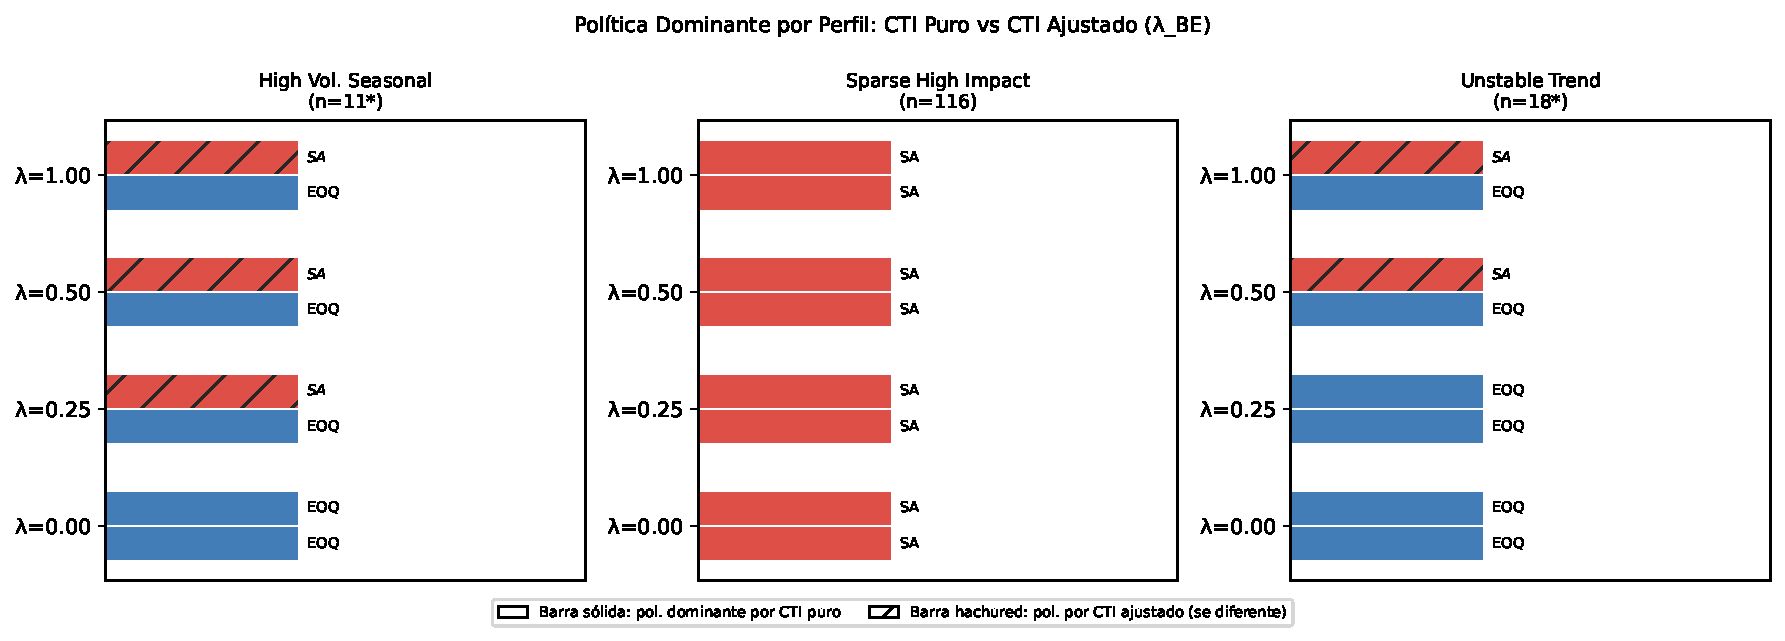
\includegraphics[width=\linewidth]{figures/cti_adjusted_sensitivity.pdf}\\
      \scriptsize Sensibilidade a $\lambda_{BE}$
    \column{0.52\textwidth}
      \small
      $J(\pi,g) = \mathrm{CTI}_{\text{norm}} + \lambda_{BE}\cdot \mathrm{BE}_{\text{norm}}$
      \vspace{0.5em}

      \begin{itemize}
        \small
        \item $\lambda_{BE}=0$: recupera o CTI puro (EOQ domina)
        \item $\lambda_{BE}\geq 0{,}25$: política única migra para
          \highlight{SA} (BE\,$=$\,5,5 vs.\ 55,4 do EOQ)
        \item Em $\lambda_{BE}=1{,}0$: até +56,6\% de redução ajustada,
          com NS caindo de 0,942 para 0,862
      \end{itemize}
  \end{columns}
  \vspace{0.4em}
  \begin{alertblock}{Status: preliminar e complementar}
    \footnotesize Não substitui o critério principal (CTI puro sob NS
    $\geq 0{,}70$). A partir de $\lambda_{BE}\geq 0{,}5$, a seleção por perfil
    converge para a política única ajustada.
  \end{alertblock}
  \note{
    Além do CTI puro, reportamos uma análise de sensibilidade que penaliza
    o custo normalizado pelo efeito bullwhip normalizado, com peso lambda.
    Com lambda zero, recuperamos exatamente o critério principal. Conforme
    lambda aumenta, a política única ótima migra do EOQ -- que tem BE muito
    alto, 55,4 -- para o SA, que é muito mais estável, com BE de 5,5,
    produzindo reduções de custo ajustado maiores, de até 56,6%, mas com
    queda adicional de nível de serviço. É fundamental destacar que essa é
    uma análise preliminar e complementar -- o critério principal da
    dissertação continua sendo o CTI puro sob a restrição de NS mínimo.
    Notem também que, quando a penalidade por instabilidade domina, a
    seleção por perfil perde sua vantagem diferenciadora, porque a política
    mais estável passa a ser preferida uniformemente em todos os perfis.
  }
\end{frame}
